\documentclass[ignorenonframetext,aspectratio=169]{beamer}

\usetheme[]{rli}

\usepackage[normalem]{ulem}
\usepackage{listings}
\lstloadlanguages{Python}
\lstset{
  % language=Python,
  basicstyle=\scriptsize\sffamily,
  numberstyle=\color{gray},
  stringstyle=\color[HTML]{933797},
  commentstyle=\color[HTML]{228B22}\sffamily,
  emph={[2]from,import,pass,return}, emphstyle={[2]\color[HTML]{DD52F0}},
  emph={[3]range}, emphstyle={[3]\color[HTML]{D17032}},
  emph={[4]for,in,def}, emphstyle={[4]\color{blue}},
  showstringspaces=false,
  breaklines=true,
  prebreak=\mbox{{\color{gray}\tiny$\searrow$}},
  numbers=left,
  xleftmargin=15pt
}

\usepackage{longtable,booktabs}
\usepackage{natbib}


\tikzset{
invisible/.style={opacity=0},
visible on/.style={alt={#1{}{invisible}}},
alt/.code args={<#1>#2#3}{%
  \alt<#1>{\pgfkeysalso{#2}}{\pgfkeysalso{#3}} % \pgfkeysalso doesn't change the path
},
}

\newsavebox{\codebox}% For storing listings

\hypersetup{
  colorlinks,
  urlcolor=rlilinkcolor
}

\title{The RLI \LaTeX{} beamer theme}
\subtitle{\ldots finally overcoming MS Powerpoint}
\author{Guido Pleßmann \and Jann Launer \and Matthias Laugwitz}
\date{\today}
\institute{Reiner Lemoine Institut}

\newcommand{\tel}{+49 (0)30 1208 434 72}
\newcommand{\email}{guido.plessmann@rl-institut.de}
\newcommand{\twitter}{\href{https://twitter.com/gplssm}{@gplssm}}
\newcommand{\finalstatement}{Enjoy stating a final statement ;-)}

\begin{document}
\frame{\titlepage}

\begin{frame}[fragile]{A new frame}
Create a new frame with title and content

\end{frame}

\begin{frame}[fragile]{Use formatting syntax}

The \emph{quick} \textbf{brown} fox \textsuperscript{jumps}
\textsubscript{over} the \texttt{lazy} \texttt{dog}\sout{, not the cat}.

You can also quote it

\begin{quote}
The quick brown fox jumps over the lazy dog, not the cat.
\end{quote}

Moreover, you can simply write \LaTeX{} code in .md files.

\end{frame}

\begin{frame}{Use lists and enumerated lists}

\begin{itemize}
\item item a

  \begin{itemize}
  \item item a.1

    \begin{itemize}
    \item item a.1.a
    \item item a.1.b
    \end{itemize}
  \end{itemize}
\end{itemize}

\begin{enumerate}
\item item 1

  \begin{enumerate}
  \item item a
  \end{enumerate}
\item item 2
\item item 3

  \begin{itemize}
  \item mix
  \item it
  \end{itemize}
\end{enumerate}

\end{frame}

\begin{frame}{Descriptions}

\begin{description}
\item[Distributed Energy Resource]
Electrical power generation or storage located at or near the point of
use, as well as demand side measures.
\item[Distributed Generation]
Electric power generation located at or near the point of use.
\item[Distributed Power]
Electrical power generation or storage located at or near the point of
use.
\end{description}

\footnotesize Content stolen from
\href{https://aceee.org/glossary_data}{ACEEE glosarry}.

\end{frame}

\begin{frame}{Insert images}
\protect\hypertarget{insert-images}{}

\center

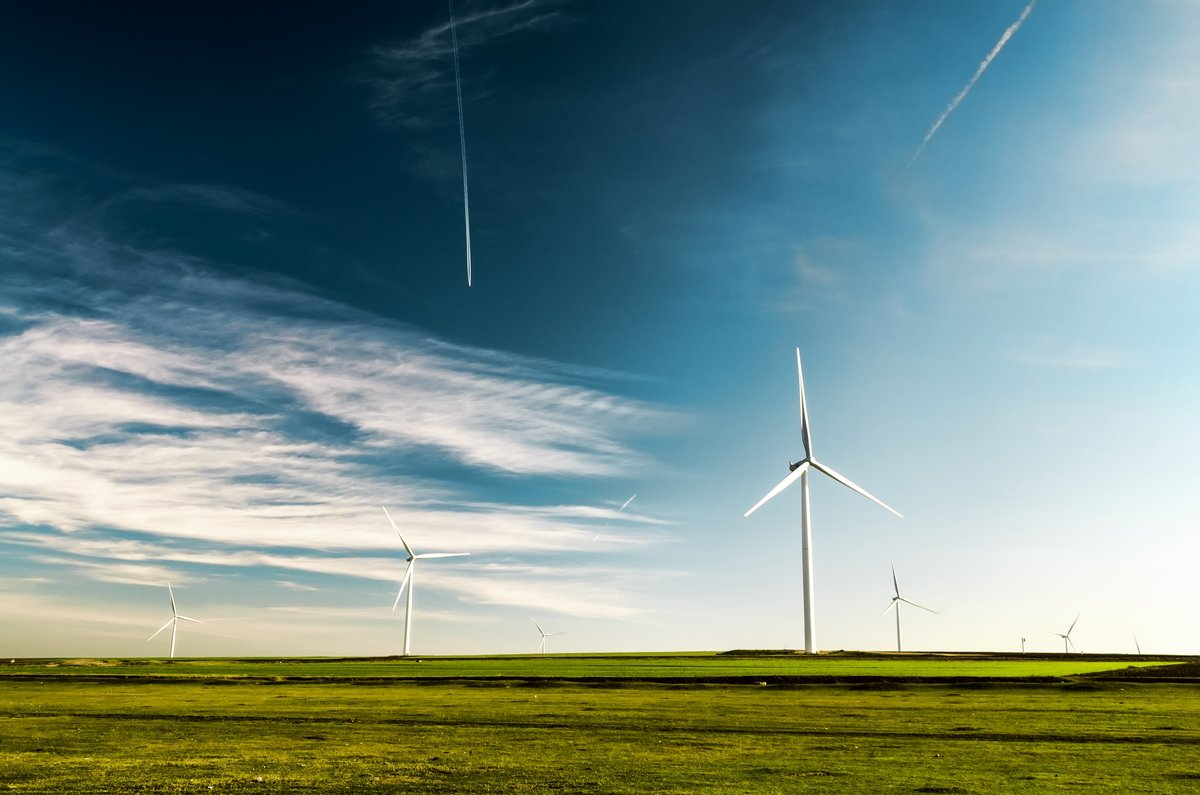
\includegraphics[width=0.75\textwidth,height=\textheight]{img/createria-ZYu6P9-Glic-unsplash_resized.jpg}

\end{frame}

\begin{frame}[fragile]{Presenting code}

\begin{lstlisting}[language=Python]
import requests
import pandas as pd
from tabulate import tabulate

df = pd.DataFrame(requests.get('http://openenergy-platform.org/api/v0\
  /schema/supply/tables/bnetza_eeg_anlagenstammdaten/rows/?limit=100').json())

df = df[[
  '4.11_bundesland',
  '4.1_energieträger', 
  '4.2_installierte_leistung',
  '4.16_name_des_netzbetreibers']]
df.columns = ["Federal state", "Technology", "Inst. Power", "Grid operator"]

print(tabulate(df.head(10), tablefmt="pipe", headers="keys"))
\end{lstlisting}

\end{frame}

\begin{frame}{Tables}

\footnotesize{
\begin{longtable}{rllrl}
\toprule
{} & Federal state & Technology & Inst. Power & Grid
operator\\
\midrule
0 & Niedersachsen & Biomasse & 366 & Avacon AG\\
1 & Bayern & Biomasse & 380 & Bayernwerk AG\\
2 & Bayern & Wasserkraft & 6 & Bayernwerk AG\\
3 & Hessen & Biomasse & 380 & EnergieNetz Mitte GmbH\\
4 & Bayern & Wind Land & 3050 & Bayernwerk AG\\
5 & Nordrhein-Westfalen & Biomasse & 400 & Westfalen Weser Netz
GmbH\\
6 & Nordrhein-Westfalen & Biomasse & 1200 & Westfalen Weser Netz
GmbH\\
7 & Schleswig-Holstein & Wind Land & 2000 & Schleswig-Holstein Netz
AG\\
8 & Hessen & Biomasse & 400 & EnergieNetz Mitte GmbH\\
9 & Bayern & Biomasse & 1000 & MDN Main-Donau Netzgesellschaft
mbH\\
\bottomrule
\end{longtable}
}
\end{frame}

\begin{frame}{Math}

\href{https://oemof.readthedocs.io/en/stable/oemof_solph.html\#oemof-solph-custom-sinkdsm-label}{SinkDSM}
following ``On the representation of demand-side management in power
system models'' \cite{ZERRAHN2015840} \vspace{-1ex} \begin{align}
\onslide<1->{\quad \dot{E}_{t} = demand_{t} + DSM_{t}^{up} - \sum_{tt=t-L}^{t+L} DSM_{t,tt}^{do}  \quad \forall t \in \mathbb{T}\\}
\onslide<2->{\quad DSM_{t}^{up} = \sum_{tt=t-L}^{t+L} DSM_{t,tt}^{do} \quad \forall t \in \mathbb{T}\\}
\onslide<3->{\quad DSM_{t}^{up} \leq  E_{t}^{up} \quad \forall t \in \mathbb{T}\\}
\onslide<4->{\quad \sum_{t=tt-L}^{tt+L} DSM_{t,tt}^{do}  \leq E_{tt}^{do} \quad \forall tt \in \mathbb{T}\\}
\onslide<5>{\quad DSM_{t}^{up}  + \sum_{t=tt-L}^{tt+L} DSM_{t,tt}^{do} \leq max \{ E_{tt}^{up}, E_{tt}^{do} \}\quad \forall tt \in \mathbb{T}\\}
\notag
\end{align}

\end{frame}

\begin{frame}{Blocks}
\begin{block}{Block header}
Block content
\end{block}
\end{frame}

\begin{frame}{Use columns to organize your content}

\begin{columns}[T]
\begin{column}{0.55\textwidth}
\includegraphics[width=\textwidth]{example-image-a}
\end{column}

\begin{column}{0.45\textwidth}
\begin{itemize}[<+->]
\item Explain
\item what's
\item to
\item see
\end{itemize}
\end{column}
\end{columns}

\end{frame}

\begin{frame}{Aligning images}

\begin{figure}
\begin{minipage}{0.3\textwidth}
\centering
\includegraphics[height=2.5cm]{example-image-a}%
\end{minipage}%
\begin{minipage}{0.3\textwidth}
\centering
\includegraphics[height=2.5 cm]{example-image-b}%
\end{minipage}%
\begin{minipage}{0.3\textwidth}
\centering
\includegraphics[height=2.5 cm]{example-image-c}%
\end{minipage}%

\vspace{5ex}

\begin{minipage}{0.45\textwidth}
\centering
\includegraphics[height=2.5 cm]{example-image-a}%
\end{minipage}%
\begin{minipage}{0.45\textwidth}
\centering
\includegraphics[height=2.5 cm]{example-image-b}%
\end{minipage}%
\end{figure}

\end{frame}

\begin{frame}{Drawing with Tikz: animated energy system block diagram}
\protect\hypertarget{drawing-with-tikz-animated-energy-system-block-diagram}{}

\begin{columns}[T]
\begin{column}{0.45\textwidth}
\begin{tikzpicture}

\tikzstyle{icon} = [inner sep=0pt];
\tikzstyle{flow} = [ultra thick, inner sep=0pt];

\coordinate (busTop) at (0.5\paperwidth,0.8\paperheight);
\coordinate (busBottom) at (0.5\paperwidth,0.3\paperheight);

\node (elecbus) at ($(busBottom) - (0,.5)$) {Household busbar};
\draw[line width=4pt](busTop) -- (busBottom);


\node[icon,draw,very thick, rounded corners=0.5ex, inner sep=3pt,visible on=<5->](dsm) at ($(busTop)!0.5!(busBottom) - (1,0)$) {{\visible<5->{
\includegraphics[width=.8cm]{img/noun_filter_1653638.pdf}}}};
\node[icon](demand) at ($(busTop)!0.5!(busBottom) - (2.5,0)$) {{\visible<2->{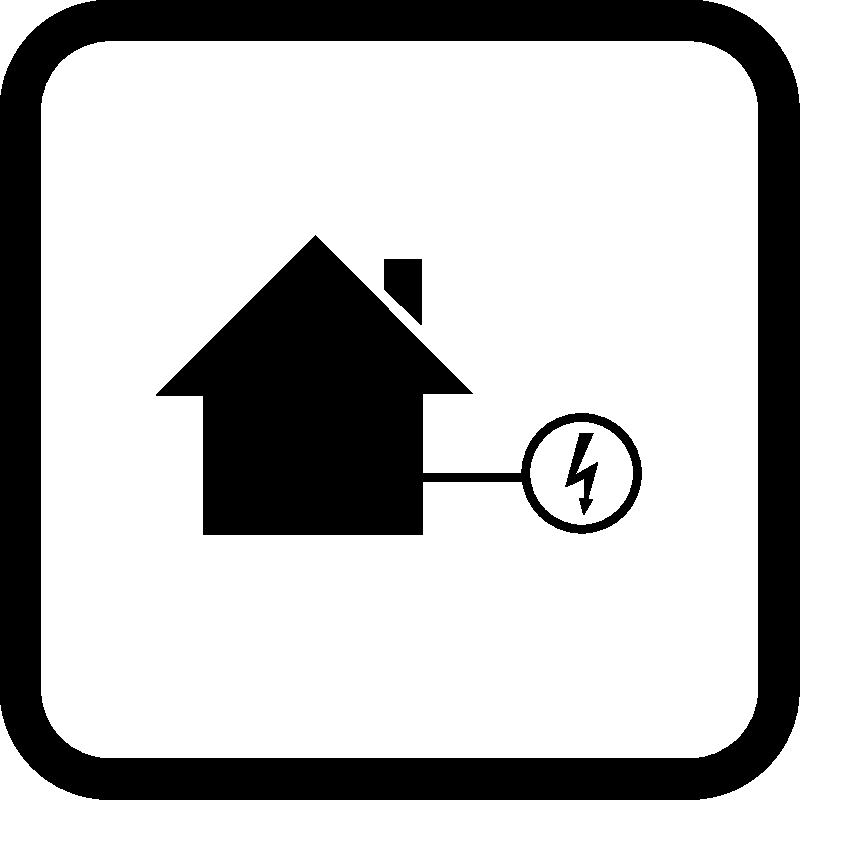
\includegraphics[width=1.1cm]{img/Verbraucher_Haushalt_Strom.pdf}}}};
\node[icon](grid) at ($(busTop)!0.7!(busBottom) + (1,0)$) {{\visible<4->{
\includegraphics[width=1.1cm]{img/Transport_Strom.pdf}}}};
\node[icon](pv) at ($(busTop)!0.3!(busBottom) + (1,0)$) {{\visible<3->{
\includegraphics[width=1.1cm]{img/Stromerzeuger_Photovoltaik_Dachanlage.pdf}}}};

\draw[<-,flow, visible on=<5->](dsm) -- ($(busTop)!0.5!(busBottom)$);
\draw[->,flow, visible on=<5->](dsm) -- (demand);
\draw[<-,flow, visible on=<4->] ($(busTop)!0.7!(busBottom) + (2pt,0)$) -- (grid);
\draw[<-,flow, visible on=<3->] ($(busTop)!0.3!(busBottom) + (2pt,0)$) -- (pv);


\end{tikzpicture}
\end{column}

\begin{column}{0.4\textwidth}
\textbf{Assuming we have a household including}

\begin{itemize}
\item<2-> Demand
\item<3-> PV
\item<4-> Grid connection
\item<5-> Demand-side management unit
\end{itemize}
\end{column}
\end{columns}

\end{frame}

\begin{frame}

Frame with no title

\end{frame}

\begin{frame}[plain]{}

\ldots or a plain one, even without footer.

\end{frame}

\begin{frame}[fragile]{How to use the theme}

\begin{itemize}
\item
  You need the \texttt{.sty} files and the \texttt{img/} folder right
  next to your \texttt{slides.md} file
\item
  Recommended workflow

  \begin{itemize}
  \item Have the clone of \url{https://github.com/rl-institut/beamer_theme/}
    \begin{lstlisting}
    gitclone git@github.com:rl-institut/beamer_theme.git}
  \end{lstlisting}
  \item Keep it up-to-date
  \item Copy required files to your slides path
    \begin{lstlisting}[language=Bash]
    cp -r beamer_theme/img/ beamer_theme/*.sty <path-of-slide.md> 
    \end{lstlisting}
  \end{itemize}
\end{itemize}

\end{frame}

\begin{frame}[fragile]{Command to build these slides}

\begin{lstlisting}[language=Bash]
xelatex example-slides.tex
\end{lstlisting}

with

\begin{lstlisting}[language=TeX]
\usetheme{rli}
\end{lstlisting}
in the preamble.
\end{frame}

\begin{frame}[fragile]{Info on last page}

Requires the following \LaTeX{} code in your preamble

\begin{lstlisting}[language=TeX]
\newcommand{\tel}{+49 (0)30 1208 434 72}
\newcommand{\email}{guido.plessmann@rl-institut.de}
\newcommand{\twitter}{\href{https://twitter.com/gplssm}{@gplssm}}
\newcommand{\finalstatement}{Enjoy stating a final statement ;-)}
\end{lstlisting}

\end{frame}

\begin{frame}{Find help}

\begin{itemize}
\item Pandoc manual: \url{https://pandoc.org/MANUAL.html}
\item Useful overview of commands for formatting with Markdown and pandoc:
  \url{http://www.flutterbys.com.au/stats/tut/tut17.3.html}
\item Theme repository: \url{https://github.com/rl-institut/beamer_theme}
\end{itemize}

\end{frame}


\begin{frame}[plain]{}

\insertendpagecontent

\end{frame}

\begin{frame}{References}
\bibliographystyle{apalike}
\bibliography{bib/example.bib} 
\end{frame}

\end{document}
